\chapter{3-Progressions and The Cap-Set Problem}\footnote{This is not a complete chapter. Instead, we only present a few problems and theorems related. }

\section{The Cap-Set Problem}
The problem goes as follows. Consider $A \subseteq \mathbb F_3^n$. Let $N = 3^n$ and $|A| \geq N / C$. How large can $C$ be so that we always have $a, b, c \in A$ such that $a + b = 2c$? Note that arithmetics are defined over finite fields here. For example if we have $\mathbb F _3^n = \{0, 1, 2\}^n$, then
\begin{itemize}
	\item $(1, 1, \dots, 1) + (2, 2, \dots, 2) = (0, \dots, 0)$
	\item $2 (2, 2, \dots, 2) = (1, 1, \dots, 1)$
\end{itemize}

This is called the Cap-Set problem because the condition we had in the original statement is such that 
\begin{equation}
	a + b = 2c \quad \iff \quad a + b + c = 0 
\end{equation}

\begin{figure}[h]
	\center
	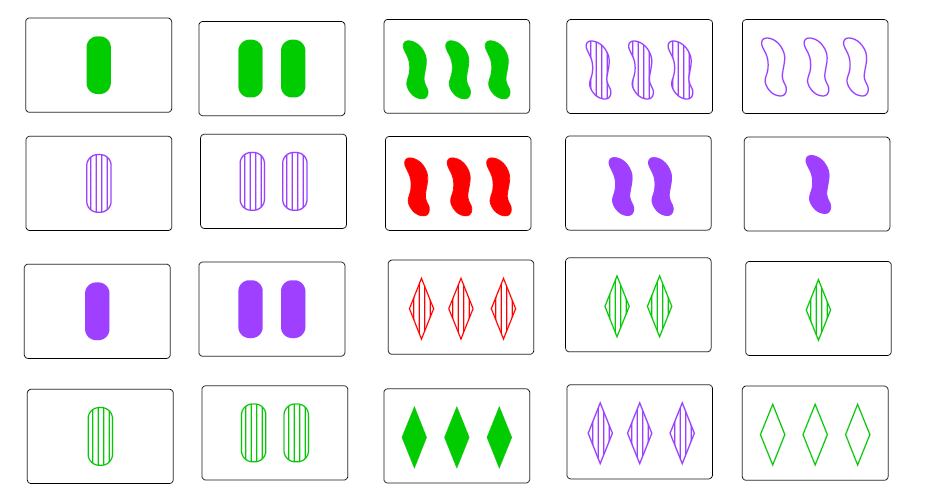
\includegraphics[width=0.6\textwidth]{figs/setgane.png}
	\caption{Tokens of the Set game (examples).}
	\label{fig:setgame}
\end{figure}
Now, this is a natural way to represent the game Set (see Figure \ref{fig:setgame}), where tokens can be represented in finite field $\mathbb F_3^4$, which constitutes the vector representation
\begin{equation}
	(number, color, shade, shape)
\end{equation} 
four items each of which has 3 possible values. The winning condition of the game is to pick three cards such that they have no intersection in this finite field representation, i.e. find three cards $a, b, c \in \mathbb F_3^4$ such that $a + b + c = 0 \in \mathbb F_3^4$. 

\paragraph{Proof Idea}
\begin{itemize}
	\item Either we already have many 3-progression. Or,
	\item We can do some ``density increment''. This is to say that $\exists$ an affine space $V$ of co-dimension $1$ where 
		\begin{equation}
			\frac{|A \cap V|}{V} > \frac{|A|}{N}
		\end{equation}
	where co-dimension is just the dimension of the complement
	\item the proof follows from induction. 
\end{itemize}

\begin{proposition}
	[Stronger Roth (Integer Version)]
	\begin{equation}
		\left( |A| \geq \frac{3^n}{n} \right) \implies \exists a, b, c, \in A \quad s.t. \quad a + b = 2c
	\end{equation}
	\label{prop:strong-roth}
\end{proposition}
This proposition is stronger than Roth's Theorem since it is over integers rather than finite field, which had nicer properties. 

\section{Fourier Characters}
Fourier characters $c$ is a set of functions
\begin{equation}
	\chi_a: \mathbb F_3^n \rightarrow \mathbb C \quad \quad \chi_a (x) = \exp \left\{ 
		\frac{2\pi i}{3} \left( \sum_{i = 1}^n a_i x_i \right)
	\right\}
\end{equation}
where $\chi_1(x) = 1, \forall x$. 

\begin{proposition}
	[Fourier Characters Properties]
	For any function on the field that we are interested on $f: \mathbb F_3^n \rightarrow \real$, we can write it as 
	\begin{equation}
		f(x) = \sum_a \hat f (a) \chi _a (x)  \quad \quad 
		\text{where}\footnote{$\hat f(a)$ is the Fourier coefficient}
		 \quad \hat f(a) = \underset{n\sim Unif(\mathbb F_3^n)}{\mathbb E} [f(n) \chi_a(n)]
	\end{equation}
	
	\paragraph{Orthogonality} Fourier characters are orthonormal to each other, i.e.,  
	\begin{equation}
		\forall a \neq b, \sum_{x \in \mathbb F _3^n} \chi_a(x) \chi_b(x) = 0
	\end{equation}
	
	\paragraph{Inner Product} The inner product between two functions
	\begin{equation}
		f, g : \mathbb F_3^n \rightarrow \real
	\end{equation}
	is equal to 
	\begin{equation}
		\langle f, g \rangle = \mathbb F_x [f(x) g(x)] = \sum_a \hat f(a) \hat g(a) = \frac{1}{3^n} \sum_x f(x)g(x)
	\end{equation}
	
	\paragraph{Convolution} The convolution between two functions $f, g : \mathbb F_3^n$ checks how correlated two functions are after a shift. Mathematically, 
	\begin{equation}
		(f\star g)(x) = \mathbb E _ y [f(y) g(x - y)]
	\end{equation}
	Now, we say $f, g$ and their coefficients are in the physical space, while $(f\star g)$ and its coefficients are in the \textbf{\textit{phase space}} or \textbf{\textit{frequency space}}.
\end{proposition}

\begin{proposition}
    [More Properties of Fourier Characters]
    For any function on the field that we are interested on $f: \mathbb F_3^n \rightarrow \real$, we can write it as 
	\begin{equation}
		f(x) = \sum_a \hat f (a) \chi _a (x)  \quad \quad 
		\text{where}\footnote{$\hat f(a)$ is the Fourier coefficient}
		 \quad \hat f(a) = \underset{n\sim Unif(\mathbb F_3^n)}{\mathbb E} [f(n) \chi_a(n)]
	\end{equation}
	Then
	\begin{itemize}
	    \item $\mathbb E_x[f(x)] = \hat f(0)$, and 
	    \item $\mathbb E_x[f(x)^2] = \sum_{a} |\hat f(a) |^2$
	\end{itemize}
\end{proposition}

\section{Proof of Proposition \ref{prop:strong-roth} (Strong Roth)}
\begin{proof}
    The original inquiry was on for $A \subseteq \mathbb F_3^n$, if there exists some $a, b, c$ such that $a + b = 2c$. Let's shift the goal a bit an instead count the number of $a, b, c$ that satisfies the condition, i.e. the quantity
    \begin{equation}
        \# = |\{a, b, c \in A : a + b = 2c \}| \equiv |\{a, b, c \in A : a + b + c = 0 \}|
    \end{equation}
    
    Obviously, if we have $\# > |A|$, then there should be three distinct elements $a, b, c \in A$ such that $a + b = 2c$. But how do we count the number of arithmetic progression? To do so, we define the indicator function 
    \begin{equation}
        \mathbb 1_A: \mathbb F_3^n \rightarrow \{0, 1\} \quad \quad \mathbb 1_A(x) = \begin{cases}
            1 & \text{ if } x \in A \\
            0 & \text{ otherwise} 
        \end{cases}
    \end{equation}
    
    Then, 
    \begin{align}
        \#
        &= |\{a, b, c \in A : a + b + c = 0 \}| \\
        &= \sum_{(a, b, c) :\, a + b + c = 0} \mathbb 1 _A(a) \cdot \mathbb 1 _A(b) \cdot \mathbb 1 _A(b) \\
        &= 3^{2n} \cdot \underset{{a, b, c \in \mathbb F_3^n \, : \, a + b + c = 0}}{\mathbb E} \left[ \mathbb 1 _A(a) \cdot \mathbb 1 _A(b) \cdot \mathbb 1 _A(b) \right]  \\
        &= (\dagger)
    \end{align}
    
    Recall the definition of convolution between two functions, where we can write it in an alternative way
    \begin{align}
        ( f\star g) (x) 
        &= \mathbb E_y [f(y) \cdot g(x - y) ] \\
        &= \mathbb E_{(a, b): a + b = x} [f(a) \cdot g(b)]
    \end{align}
    
    With convolution, we can transform $(\dagger)$ into
    \begin{equation}
        (\dagger) = 3^{2n} \mathbb 1 _A \star \mathbb 1 _A \star \mathbb 1 _A (0)
    \end{equation}
    
    Claim: (we won't show the first step).
    \begin{align}
        |\{a, b, c \in A : a + b + c = 0 \}| 
        &= 3^{2n} \cdot \sum_a \hat 1 _A (a)^3 \\
        &= 3^{2n} \cdot (\hat 1 (0)) + 3^{2n} \sum_{a \neq 0} (\hat 1 _A (a))^3
    \end{align}
    
    which according to our parametrization is 
    \begin{equation}
        \hat 1 _A(0) = \mathbb E _x [ 1_A(x)] = \frac{|A|}{N} \triangleq \delta
    \end{equation}
    
    Then, 
    \begin{align}
        \hat 1 _A(0) = 3^{2n} \delta^3 + 3^{2n} \cdot \sum_{a \neq 0} 1_A (a)
    \end{align}
    
    Hence so far we know 
    \begin{align}
        3\# - e^{2n} \cdot \delta ^3 
        &= 3^{2n} \cdot \sum_{a \neq 0} \hat 1_A(a)^3 \\
        &\leq 3^{2n} \cdot \sum_{a \neq 0} |\hat 1 A(a)|^3 \\
        &= 3^{2n} \cdot \left(\sum_{a \neq 0} |\hat 1_A (a)| ^2\right) \cdot \left(\max_{b \neq 0} 1_A(b)\right)
    \end{align}
    
    Now, 
    \begin{align}
        \delta
        &= \mathbb E_x [1_A(x)] \\
        &= \mathbb E_x [1_A(x)^2] \\
        &= \sum_a |\hat 1 (a)|^2 \\
        &= \hat 1 _A(0)^2 + \sum_{a \neq 0} |\hat 1 _A (a)|^2 
    \end{align}
    
    where we can put this back in
    \begin{align}
        &|3 \cdot \# -3^{2n} \cdot \delta^3|
        \leq 3^{2n} \cdot \left( \max_{b \neq 0} |\hat 1 _A(b)| \right) \cdot (\delta - \delta^2 ) \\
        \implies & \max_{b \neq 0} |\hat 1 _A(b)| \geq \frac{|3 \cdot \# -3^{2n} \cdot \delta^3|}{\delta - \delta^2}
    \end{align}
    
    We proceed with the proof with induction. If $3\# > 3^n \cdot \delta$, then we are good. Otherwise, we know we know the inequality that we derived above 
    \begin{align}
        \max_{b \neq 0} |\hat 1 _A(b)| 
        &\geq \frac{|3 \cdot \# -3^{2n} \cdot \delta^3|}{\delta - \delta^2} \\
        &= \frac{|3^{2n} \cdot \delta^3 - 3 \cdot \#|}{\delta - \delta^2} \\
        &\geq \frac{3^{2n} \cdot \delta^3 - 3^n\cdot \delta}{3^{2n} \cdot (\delta - \delta^2)} \\
        &\approx \frac{\delta^2}{2}
    \end{align}
    
    This implies on one of the following three spaces, we have $\frac{|A\cap U|}{|V|} \geq \delta + \Omega(\delta^2)$. 
    
    The three affine spaces are the following
    \begin{equation}
        \begin{matrix}
            \{x : \langle b^\star, x \rangle = 0  \} \\
            \{x : \langle b^\star, x \rangle = 1  \} \\
            \{x : \langle b^\star, x \rangle = 2  \}
        \end{matrix}
    \end{equation}
    
    which concludes the proof. \qed
\end{proof}
